%%%%%%%%%%%%%%%%%%%%%%%%%%%%%%%%%%%%%%%%%%%%%%%%%%%%%%%%%%
% # Appendix: Park and Choi C-Test
%%%%%%%%%%%%%%%%%%%%%%%%%%%%%%%%%%%%%%%%%%%%%%%%%%%%%%%%%%

\chapter{Park and Choi C-Test}\label{app-parkchoi}

A modified version of Park and Choi's (\citeyear{park.choi2018}) C-test was included in the C-test validation study. Participants were all L1-Korean L2ers of English (KLEs). Alterations to the original C-test are displayed in the colored boxes below. Added text is shown in green boxes with solid borders and deleted text is shown in red boxes with dashed borders. These changes were made to increase naturalness and to avoid unnecessary references to specific cultural stereotypes.

\vspace{0.5cm}

\begin{tikzpicture}
  \node[fill=red!20!white, draw=red, dashed, line width=0.6pt] (box) {
    \begin{minipage}{\textwidth}
      \textbf{Instructions:} Fill in one word in each blank. You may write directly on the test. Complete the texts in the order (TEXT 1 \rightarrow TEXT 2 \rightarrow TEXT 3).
      
      \vspace{0.5cm}
      
      \textbf{Example:} The girl was walking d\gap[align=left]{own} the street when she stepped on some ice and fell.
    \end{minipage}
  };
\end{tikzpicture}

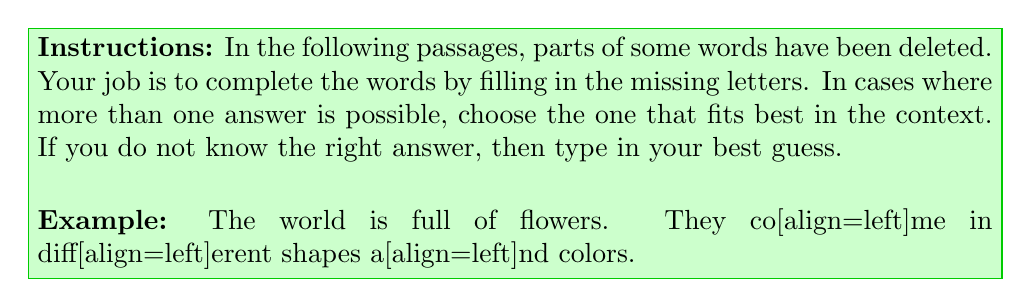
\begin{tikzpicture}
  \node[fill=green!20!white, draw=green!80!black, line width=0.6pt] (box) {
    \begin{minipage}{\textwidth}
      \textbf{Instructions:} In the following passages, parts of some words have been deleted. Your job is to complete the words by filling in the missing letters. In cases where more than one answer is possible, choose the one that fits best in the context. If you do not know the right answer, then type in your best guess.
      
      \vspace{0.5cm}
      
      \textbf{Example:} The world is full of flowers. They co\gap[align=left]{me} in diff\gap[align=left]{erent} shapes a\gap[align=left]{nd} colors.
    \end{minipage}
  };
\end{tikzpicture}

\vspace{0.5cm}

\begin{spacing}{1.2}

\textbf{Passage 1:} Steven loved almost everything about his grandma. There was only one thing he hated. She always knitted sweaters for h\gap{1}. Steven understood that she did it to be n\gap{2}. However, all the sweaters were very ugly. Steven v\gap{3} her once a week. She had a new s\gap{4} for him each time. Steven lived in a s\gap{5} apartment. There was no room for him to k\gap{6} all the sweaters. He had to give all of them a\gap{7}. “Grandma will never find out,” he thought. One d\gap{8}, Steven's grandma visited him by surprise. She asked to s\gap{9} his sweaters. “Someone stole all of them!” he s\gap{10}. “They were too nice.” She m\gap{11} him ten more by the next month.

\vspace{0.5cm}

\textbf{Passage 2:} Depression is a serious but treatable disorder that affects millions of people, from young to old and from rich to poor. It gets in the way of everyday l\gap{12}, causing tremendous pain, hurting not just those suffering f\gap{13} it, but also impacting everyone around them. If s\gap{14} you love is depressed, you may be e\gap{15} any number of difficult emotions, including helplessness, frustration, a\gap{16}, fear, guilt, and sadness. These feelings are all n\gap{17}. It's not easy dealing with a friend or f\gap{18} member's depression. And if you don't take care of y\gap{19}, it can become overwhelming. That said, there are s\gap{20} you can take to help your loved one. Start by learning about depression and how to talk a\gap{21} it with your friend or family member. But as you reach out, don't forget to l\gap{22} after your own emotional h\gap{23}. Thinking about your own needs is not an a\gap{24} of selfishness---it's a necessity. Your emotional strength will a\gap{25} you to provide the ongoing support your depressed friend or family member needs.

\vspace{0.5cm}

\textbf{Passage 3:} Nonverbal communication includes facial expressions, gestures, the distance between speakers, eye contact, voice intonations, touch, and many other minor details which can provide speakers with valuable \remove{details}\add{information} about each other. For example, \add{the amount of} s\gap{26} between people can say a lot about the level of intimacy between them: usually, the s\gap{27} the distance between speakers, the more friendly or i\gap{28} they are, and vice versa. Or if a person a\gap{29} eye contact, it might mean that he or she is hiding something, feels u\gap{30} around you, and so on. Body l\gap{31} has several important functions. For instance, a person's g\gap{32} can repeat the message he or she is m\gap{33} orally; a little child explaining how birds f\gap{34} and waving his or her arms like w\gap{35} is a decent example of this function. Another function, substitution, occurs when v\gap{36} messages can be expressed by nonverbal means (like shrugging). I\gap{37} addition, gestures can be used for accenting, like when r\gap{38} one's index finger when speaking about s\gap{39} important. At the same time, it is important to remember that sometimes body language may d\gap{40} depending on culture. For example, in some \remove{eastern} countries, l\gap{41} straight in the eyes of a conversationalist is considered r\gap{42}. Men in some \remove{Arabic countries}\add{parts of the world} may walk around the street h\gap{43} hands, or may kiss each other on the c\gap{44} when greeting, but this is \remove{the}\add{an} i\gap{45} of friendship, not romance or intimacy.

\end{spacing}

\vspace{0.5cm}

\textbf{Answers:} (1)~him, (2)~nice, (3)~visited, (4)~sweater, (5)~small, (6)~keep, (7)~away, (8)~day, (9)~see, (10)~said, (11)~made, (12)~life, (13)~from, (14)~someone, (15)~experiencing, (16)~anger, (17)~normal/natural, (18)~family, (19)~yourself, (20)~steps, (21)~about, (22)~look, (23)~health, (24)~act, (25)~allow, (26)~space, (27)~shorter/smaller, (28)~intimate, (29)~avoids, (30)~uncomfortable/uneasy, (31)~language, (32)~gestures, (33)~making, (34)~fly, (35)~wings, (36)~verbal, (37)~in, (38)~raising, (39)~something, (40)~differ, (41)~looking, (42)~rude, (43)~holding, (44)~cheek(s), (45)~indication

\newpage

%========================================================%
\section{Korean instructions}
%========================================================%

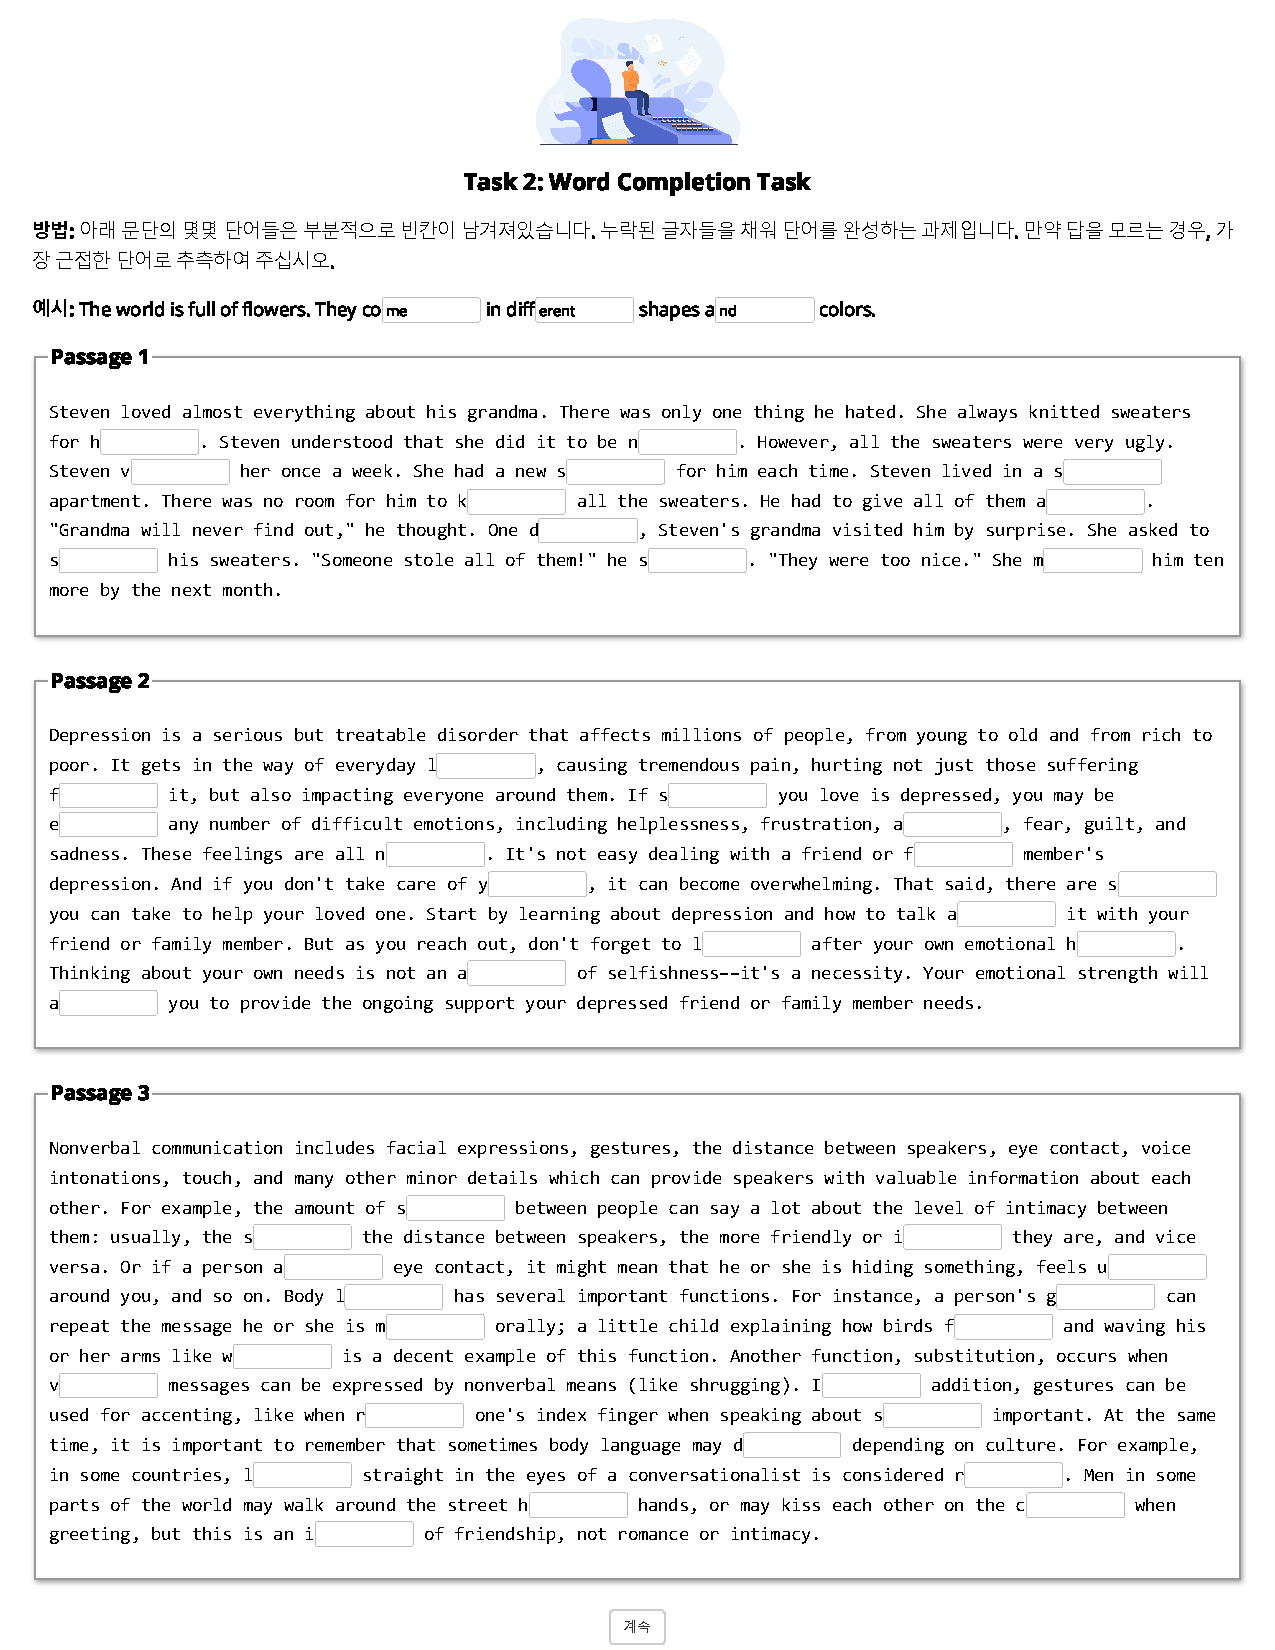
\includegraphics{../materials/instructions/ko-ct-pc.pdf}